
\chapter{Introduction}
\label{intro}

\section{Graphics \& Light}
At its core, computer graphics is the visualization of light and its interaction in an abstract world, be this a simulation or a virtual world created by artists.  The ability to render scenes with realistic lighting is desirable for many entertainment application settings such as film.  Even in non-photo-realistic renders, the interaction of light is of paramount importance.

\section{Global Illumination}
The effort to accurately evaluate the radiometric quantities within a virtual scene, especially in non-real-time systems, may be referred to collectively as \textit{global illumination} \cite{verth:2008}.  In order to achieve greater realism, scenes must rely on more than simple direct-lighting algorithms and move to more complex systems to better evaluate light interaction (Figure \ref{fig:cornell}.)  This field of study has lent itself to the breathtaking visual effects in movies, advertisements, television shows and other artistic mediums.  The line between real and fake is getting blurrier every year as the lighting calculations become more and more exact.  As we have pushed the boundaries of our graphical capabilities, we also increase our computational complexity exponentially.

\begin{figure}[h!]
    \centering
    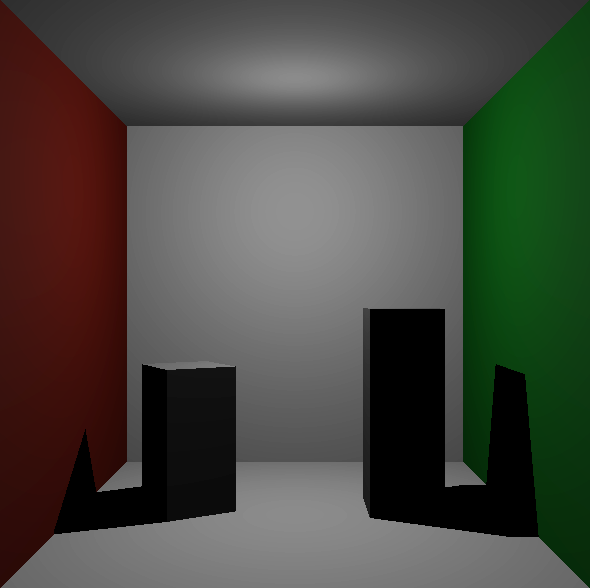
\includegraphics[width=70mm]{../img/boxes_noindirect.png}
    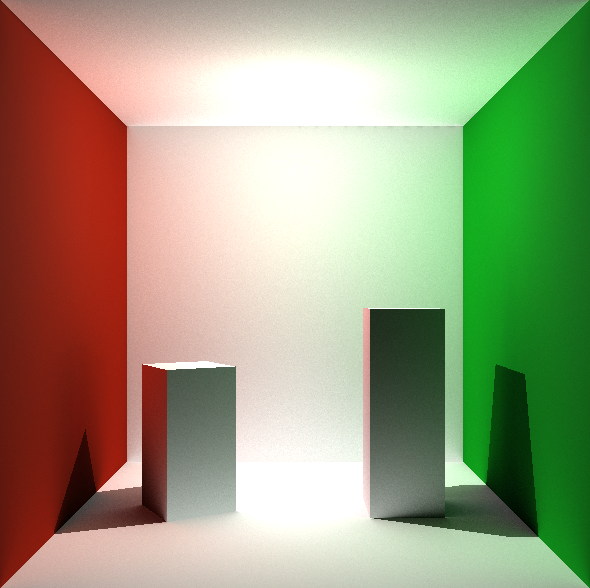
\includegraphics[width=70mm]{../img/indirect_box_high.png}
    \captionfonts
    \caption{A simple Cornell box scene with direct lighting only (left) and the same scene showing single-bounce light interaction through a global illumination algorithm (right.)}
    \label{fig:cornell}
\end{figure}

\section{Color Bleeding Techniques}

Great results have been achieved for lighting complex scenes using point based color bleeding~\cite{christensen:2008} algorithms, where a point-cloud representation of a scene's direct lighting is computed for the purpose of efficiently calculating a representation of the scene's radiometric properties surrounding any given point.  Per H. Christensen's color bleeding algorithm (or similar implementations) is already in place in many production companies and used in many feature films.

These algorithms, however, tend to limit or omit entirely the lighting contribution from volumetric data or participating media within the scenes.  Due to the highly complex nature of the domain, coupled with the computational complexity involved therein, many algorithms choose to disregard this portion of the lighting algorithm, often leaving the programmer or artist to fake the volume's contribution in other ways.


\section{Our Contribution}

This paper presents an algorithm to address this missing component in the point based color bleeding algorithm.  Specifically, we propose the addition of a data representation tuned to volumes,  \emph{light-voxel (or lvoxel)} to address the need to represent participating media to an existing global illumination algorithm which leverages a point cloud representation of a scene.  Over the course of this paper, we will:

\begin{enumerate}
\item Discuss the surrounding subjects of light, volume rendering and global illumination,
\item List and describe existing algorithms and related work,
\item Describe how our algorithm meets our requirements and
\item Analyze the results of our implementation.
\end{enumerate}

Our method achieves results comparable to those produced with Monte Carlo ray tracing but with drastically reduced run times, speeding up renders by a factor of 10.  Figure~\ref{fig:compare} clearly illustrates a close comparison of our algorithm and Monte Carlo ray traced results.

\begin{figure}[h!]
    \centering
    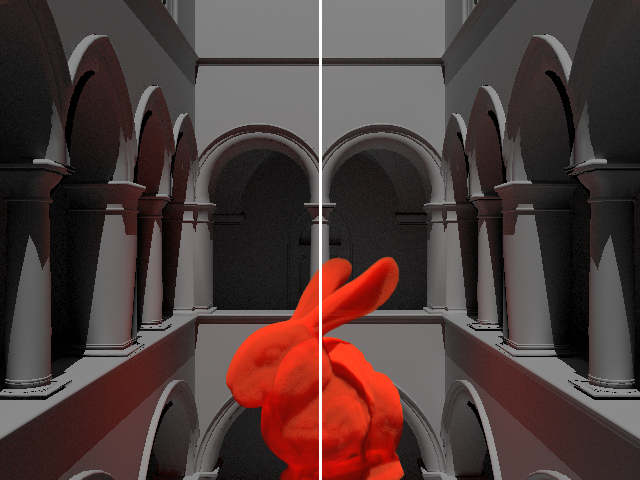
\includegraphics[width=100mm]{../img/compare.png}
    \caption{Bunny Scene comparison of the PCB extension (left) and traditional Monte Carlo results (right.)}
    \label{fig:compare}
\end{figure}
